\documentclass[12pt]{article}

\usepackage{fontspec}
\newfontfamily\handwriting{a-casual-handwritten-pen}[Path=../assets/fonts/,Extension=.ttf,Scale=1.5]
\newfontfamily\comic{Comic Neue}

\usepackage[utf8]{inputenc}
\usepackage{amsmath}
\usepackage{amssymb}
\usepackage{enumitem}
\usepackage{xcolor}
\usepackage{soul}
\usepackage{tikz}
\usepackage[most]{tcolorbox}
\usepackage{titlesec}
\usepackage{multicol}
\usepackage{environ}

\usetikzlibrary{fit, positioning, arrows.meta, decorations.pathreplacing}

% --- Custom Colors ---
\definecolor{primaryblue}{RGB}{42, 111, 151}
\definecolor{exbg}{RGB}{255, 240, 245}
\definecolor{rulebg}{RGB}{232, 245, 233}
\definecolor{highlight}{RGB}{255, 243, 176}
\definecolor{pinkanno}{RGB}{255, 105, 180}
\definecolor{purpleanno}{RGB}{147, 112, 219}
\definecolor{solutionbg}{RGB}{245, 245, 255}

% --- Header Styling ---
\titleformat{\section}{\color{primaryblue}\normalfont\Large\bfseries}{\thesection}{1em}{}
\titleformat{\subsection}{\color{primaryblue}\normalfont\large\bfseries}{\thesubsection}{1em}{}

% --- Friendly Boxes ---
% --- Auto-numbered Example Box ---
\newcounter{examplenum}

\newtcolorbox{friendlyexbox}[1]{
    colback=exbg,
    colframe=pinkanno!50,
    arc=5pt,
    title=\textbf{#1},
    coltitle=black,
    attach title to upper,
    after title={:\quad}
}

\newenvironment{friendlyex}{%
    \refstepcounter{examplenum}%
    \begin{friendlyexbox}{Example \theexamplenum}%
}{%
    \end{friendlyexbox}%
}

\newtcolorbox{friendlyrule}[1]{
    colback=rulebg,
    colframe=primaryblue!30,
    arc=5pt,
    fonttitle=\bfseries,
    title={#1},
    coltitle=primaryblue
}

\newcommand{\funhl}[1]{\sethlcolor{highlight}\hl{#1}}

% --- Show/Hide Solutions ---
\newif\ifshowsolutions

% Uncomment the next line to show solutions.
\showsolutionstrue

\newcommand{\solutionblank}{\vspace{25ex}}

\NewEnviron{solutionbox}{
\ifshowsolutions
\begin{tcolorbox}[
    colback=solutionbg,
    colframe=purpleanno!45,
    arc=5pt,
    title={Solution},
    coltitle=primaryblue,
    fonttitle=\bfseries
]
\BODY
\end{tcolorbox}
\else
\solutionblank
\fi
}

\begin{document}
\handwriting

\begin{center}
    \Large\textbf{\color{primaryblue}Module 4 Lesson 1\\Exponential Functions} \\
    \vspace{0.2cm}
    \hrule
\end{center}

\section*{Objectives}

\begin{friendlyrule}{In this lesson, we will learn how to}
\begin{itemize}
    \item identify the initial value and growth/decay factor of an exponential function;
    \item graph exponential functions and their transformations;
    \item apply exponential functions to compound interest, population growth, depreciation, and logistic growth;
    \item determine an exponential function from given data.
\end{itemize}
\end{friendlyrule}

\section*{1. A Motivating Example}

Suppose you are offered a one-month temporary job. Would you choose to be paid \$500 per day, or start at \$0.01 on the first day with your pay doubling each day?

\begin{friendlyrule}{Answer}
Choose \$0.01 doubling each day --- by Day 30 it grows to \$5{,}368{,}709.12, far more than $500\times30=\$15{,}000$.
\end{friendlyrule}

\begin{center}
{\small
\begin{tabular}{|c|c||c|c|}
\hline
Day & Amount & Day & Amount \\
\hline
1 & \$0.01 & 16 & \$327.68 \\
2 & \$0.02 & 17 & \$655.36 \\
3 & \$0.04 & 18 & \$1{,}310.72 \\
4 & \$0.08 & 19 & \$2{,}621.44 \\
5 & \$0.16 & 20 & \$5{,}242.88 \\
6 & \$0.32 & 21 & \$10{,}485.76 \\
7 & \$0.64 & 22 & \$20{,}971.52 \\
8 & \$1.28 & 23 & \$41{,}973.04 \\
9 & \$2.56 & 24 & \$83{,}886.08 \\
10 & \$5.12 & 25 & \$167{,}772.16 \\
11 & \$10.24 & 26 & \$335{,}544.32 \\
12 & \$20.48 & 27 & \$671{,}088.64 \\
13 & \$40.96 & 28 & \$1{,}342{,}177.28 \\
14 & \$81.92 & 29 & \$2{,}684{,}354.56 \\
15 & \$163.84 & 30 & \$5{,}368{,}709.12 \\
\hline
\end{tabular}
}
\end{center}

Initial value: $a=0.01$. \qquad Growth factor: $b=2$.

\[
\boxed{f(x)=0.01(2)^x}
\]

represents the salary on day $x$ since the start of the job.

\section*{2. General Form}

\begin{friendlyrule}{Exponential Function}
\[
f(x)=ab^x, \qquad \text{where } b>0 \text{ and } b\neq 1.
\]
Here $a$ is the \funhl{initial value} of $f$, since $f(0)=a$, and $b$ is the \funhl{growth or decay factor}. The function \funhl{grows} if $b>1$ and \funhl{decays} if $0<b<1$.
\end{friendlyrule}

\begin{friendlyex}{}
Identify the initial value and growth/decay factor.
\begin{enumerate}[label=(\alph*)]
    \item $f(x)=15(3)^x$
    \item $g(x)=1000\left(\dfrac12\right)^x$
    \item $h(x)=2^x$
\end{enumerate}
\end{friendlyex}

\begin{solutionbox}
\textbf{(a)} Initial value: $15$. \quad Growth factor: $3$.

\textbf{(b)} Initial value: $1000$. \quad Decay factor: $\dfrac12$.

\textbf{(c)} $h(x)=2^x=1(2)^x$. Initial value: $1$. \quad Growth factor: $2$.
\end{solutionbox}

\begin{friendlyex}{}
The following are \textbf{not} exponential functions --- give a reason why.
\begin{enumerate}[label=(\alph*)]
    \item $f(x)=1^x$
    \item $g(x)=4x^3$
    \item $h(x)=5\left(-\dfrac12\right)^x$
\end{enumerate}
\end{friendlyex}

\begin{solutionbox}
\textbf{(a)} Not exponential, because the base $b=1$ (the requirement is $b\neq 1$).

\textbf{(b)} Not exponential --- this is a \textbf{polynomial} function (the variable is in the base, not the exponent).

\textbf{(c)} Not exponential, because the base $b=-\dfrac12$ is negative; the base of an exponential function cannot be negative.
\end{solutionbox}

\section*{3. Graphs of Exponential Functions}

\textbf{$f(x)=ab^x$ with $b>1$ (growth):}

\begin{center}
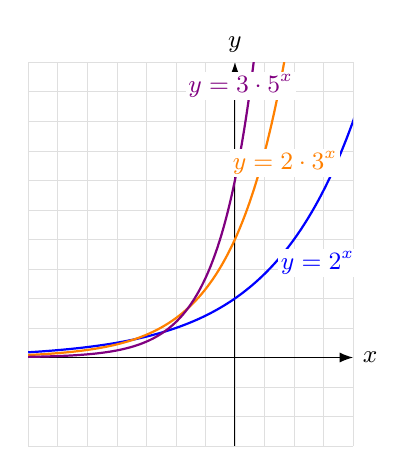
\begin{tikzpicture}[scale=0.75]
\draw[step=0.5, gray!25, very thin] (-3.5,-1.5) grid (2,5);
\draw[-{Latex}] (-3.5,0) -- (2,0) node[right] {\small $x$};
\draw[-{Latex}] (0,-1.5) -- (0,5) node[above] {\small $y$};
\begin{scope}
\clip (-3.5,-1.5) rectangle (2,5);
\draw[blue, thick, domain=-3.5:2.6, samples=80, smooth] plot (\x, {2^\x});
\draw[orange, thick, domain=-3.5:1.9, samples=80, smooth] plot (\x, {2*3^\x});
\draw[violet, thick, domain=-3.5:1.55, samples=80, smooth] plot (\x, {3*5^\x});
\end{scope}
\node[blue, fill=white, inner sep=1pt] at (1.4,1.6) {\small $y=2^x$};
\node[orange, fill=white, inner sep=1pt] at (0.85,3.3) {\small $y=2\cdot3^x$};
\node[violet, fill=white, inner sep=1pt] at (0.1,4.6) {\small $y=3\cdot5^x$};
\end{tikzpicture}
\end{center}

\textbf{$f(x)=ab^x$ with $0<b<1$ (decay):}

\begin{center}
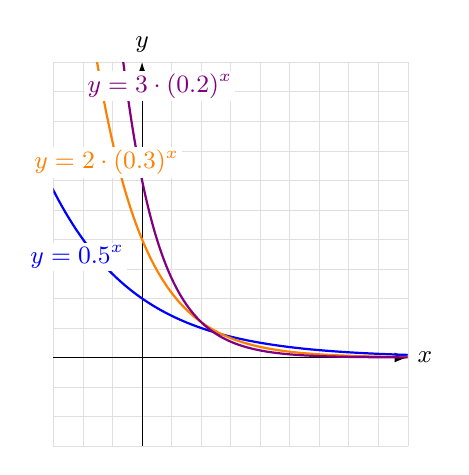
\begin{tikzpicture}[scale=0.75]
\draw[step=0.5, gray!25, very thin] (-1.5,-1.5) grid (4.5,5);
\draw[-{Latex}] (-1.5,0) -- (4.5,0) node[right] {\small $x$};
\draw[-{Latex}] (0,-1.5) -- (0,5) node[above] {\small $y$};
\begin{scope}
\clip (-1.5,-1.5) rectangle (4.5,5);
\draw[blue, thick, domain=-2.6:4.5, samples=80, smooth] plot (\x, {0.5^\x});
\draw[orange, thick, domain=-1.9:4.5, samples=80, smooth] plot (\x, {2*0.3^\x});
\draw[violet, thick, domain=-1.55:4.5, samples=80, smooth] plot (\x, {3*0.2^\x});
\end{scope}
\node[blue, fill=white, inner sep=1pt] at (-1.1,1.7) {\small $y=0.5^x$};
\node[orange, fill=white, inner sep=1pt] at (-0.6,3.3) {\small $y=2\cdot(0.3)^x$};
\node[violet, fill=white, inner sep=1pt] at (0.3,4.6) {\small $y=3\cdot(0.2)^x$};
\end{tikzpicture}
\end{center}

\section*{4. Transformations of Exponential Graphs}

\begin{friendlyex}{}
Use the graph of $y=2^x$ to graph $r(x)=2^{x-3}+1$, and determine the domain, range, and horizontal asymptote of $r(x)$.
\end{friendlyex}

\begin{solutionbox}
The graph of $r(x)$ is $y=2^x$ shifted \textbf{$3$ units right} and \textbf{$1$ unit up}.

\begin{center}
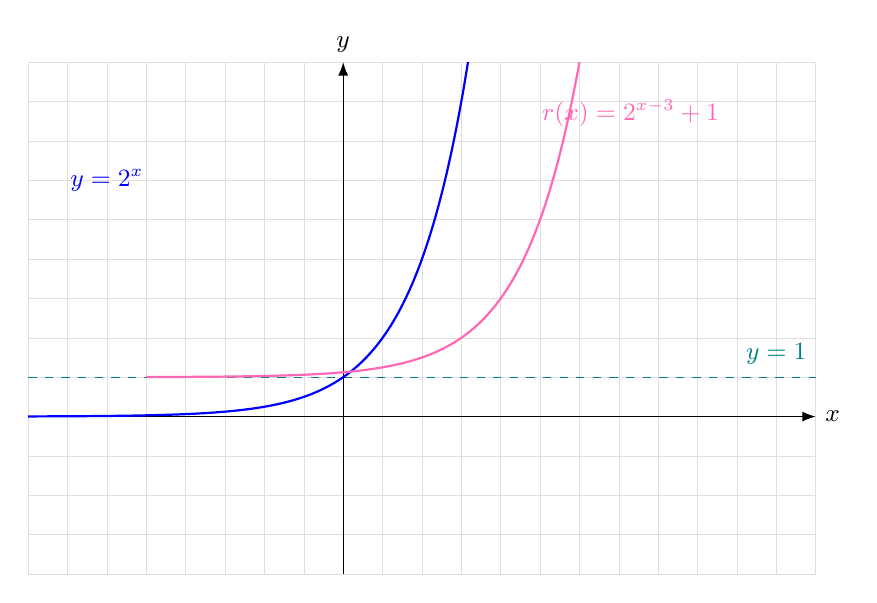
\begin{tikzpicture}[scale=0.5]
\draw[step=1, gray!25, very thin] (-8,-4) grid (12,9);
\draw[-{Latex}] (-8,0) -- (12,0) node[right] {\small $x$};
\draw[-{Latex}] (0,-4) -- (0,9) node[above] {\small $y$};
\draw[dashed, teal] (-8,1) -- (12,1);
\node[teal] at (11,1.6) {\small $y=1$};
\begin{scope}
\clip (-8,-4) rectangle (12,9);
\draw[blue, thick, domain=-8:3.2, samples=80, smooth] plot (\x, {2^\x});
\end{scope}
\node[blue] at (-6,6) {\small $y=2^x$};
\begin{scope}
\clip (-8,-4) rectangle (12,9);
\draw[pinkanno, thick, domain=-5:9.2, samples=80, smooth] plot (\x, {2^(\x-3)+1});
\end{scope}
\node[pinkanno] at (7.3,7.7) {\small $r(x)=2^{x-3}+1$};
\end{tikzpicture}
\end{center}

\textbf{(a) Domain of $r(x)$:} $(-\infty,\infty)$, all real numbers.

\textbf{(b) Range of $r(x)$:} $(1,\infty)$.

\textbf{(c) Horizontal Asymptote:} $y=1$.
\end{solutionbox}

\section*{5. Applications of Exponential Functions}

\subsection*{Compound Interest}

\begin{friendlyrule}{Compound Interest Formulas}
If $P$ dollars (principal) is invested at annual rate $r$ (decimal form), the amount $A$ in the account after $t$ years is:
\begin{itemize}
    \item For $n$ compounding periods per year: \quad $A=P\left(1+\dfrac{r}{n}\right)^{nt}$
    \item For continuous compounding: \quad $A=Pe^{rt}$
\end{itemize}
\end{friendlyrule}

\begin{friendlyex}{}
\$1000 is invested at 5\% interest compounded monthly. How much money is in the account after 3 years?
\end{friendlyex}

\begin{solutionbox}
$P=1000,\ r=0.05,\ n=12,\ t=3$.
\[
A=P\left(1+\frac{r}{n}\right)^{nt}=1000\left(1+\frac{0.05}{12}\right)^{(12)(3)}\approx \boxed{\$1161.47}
\]
\end{solutionbox}

\begin{friendlyex}{}
\$1000 is invested at 5\% interest compounded continuously. How much money is in the account after 3 years?
\end{friendlyex}

\begin{solutionbox}
$P=1000,\ r=0.05,\ t=3$.
\[
A=Pe^{rt}=1000e^{(0.05)(3)}\approx \boxed{\$1161.83}
\]
\end{solutionbox}

\subsection*{Population Growth}

\begin{friendlyrule}{Population Growth Formula}
Given an initial population $P_0$ and annual growth rate $r$ (decimal), the population after $t$ years is
\[
P(t)=P_0e^{rt}.
\]
\end{friendlyrule}

\begin{friendlyex}{}
A small town's population is modeled by $P(t)=11500e^{0.025t}$, where $t$ is the number of years since 2020.
\begin{enumerate}[label=(\alph*)]
    \item Initial population of the town.
    \item Annual growth rate in percentage.
    \item Population of the town in 2030.
\end{enumerate}
\end{friendlyex}

\begin{solutionbox}
\textbf{(a)} Initial population: $P_0=11{,}500$.

\textbf{(b)} Annual growth rate: $r=0.025=2.5\%$.

\textbf{(c)} From 2020 to 2030, $t=10$ years:
\[
P(10)=11500\,e^{(0.025)(10)}\approx \boxed{14{,}766 \text{ people}}
\]
\end{solutionbox}

\subsection*{Depreciation}

\begin{friendlyrule}{Depreciation Formula}
If an item purchased new at price $V_0$ depreciates at annual rate $r$ (decimal), its value $t$ years after purchase is
\[
V=V_0(1-r)^t.
\]
\end{friendlyrule}

\begin{friendlyex}{}
An automobile bought new at \$27{,}500 depreciates $6\%$ annually.
\begin{enumerate}[label=(\alph*)]
    \item Find the formula for the value $t$ years after purchase.
    \item What is the value of the car $4$ years after purchase?
    \item How long will it take for the car to be worth only \$15{,}000? Set up the equation.
\end{enumerate}
\end{friendlyex}

\begin{solutionbox}
\textbf{(a)}
\[
V=V_0(1-r)^t=27500(1-0.06)^t=\boxed{27500(0.94)^t}
\]

\textbf{(b)} At $t=4$:
\[
V=27500(0.94)^4\approx \boxed{\$21{,}080.22}
\]

\textbf{(c)} Set $V=15000$:
\[
\boxed{15000=27500(0.94)^t}
\]
(This equation is solved using logarithms --- see Lesson 4.4.)
\end{solutionbox}

\subsection*{Logistic Growth}

\begin{friendlyex}{}
At a school of $10{,}000$ students, one student returns from Spring break with a contagious flu virus. The spread of the virus is modeled by
\[
N=\frac{10000}{1+9999e^{-0.6t}},
\]
where $N$ is the number of students infected after $t$ days.
\begin{enumerate}[label=(\alph*)]
    \item How many students are infected after $5$ days?
    \item The college will cancel classes if $50\%$ of the students are infected --- when might that occur? Set up the equation.
\end{enumerate}
\end{friendlyex}

\begin{solutionbox}
\textbf{(a)} Substitute $t=5$:
\[
N=\frac{10000}{1+9999e^{-0.6(5)}}\approx \boxed{20 \text{ students}}
\]

\textbf{(b)} $50\%$ of $10{,}000$ is $5000$, so set $N=5000$:
\[
\boxed{5000=\frac{10000}{1+9999e^{-0.6t}}}
\]
(This equation is solved using logarithms --- see Lesson 4.4.)
\end{solutionbox}

\section*{6. Determining an Exponential Function from Data}

\begin{friendlyrule}{Strategy}
Start with $f(x)=ab^x$. Substitute two known input/output pairs to get two equations, then divide one equation by the other to eliminate $a$ and solve for $b$; finally substitute back to find $a$.
\end{friendlyrule}

\begin{friendlyex}{}
An insect population starts at $65$ and grows exponentially. After $3$ days, the population is $1755$. Find the function $P(t)$ that models this growth, where $t$ is the number of days.
\end{friendlyex}

\begin{solutionbox}
Let $P(t)=ab^t$. We are given $a=65$ (the initial value) and $P(3)=1755$:
\[
P(3)=65b^3 \implies 1755=65b^3 \implies \frac{1755}{65}=b^3 \implies 27=b^3.
\]
\[
3^3=b^3 \implies b=3.
\]
\[
\boxed{P(t)=65(3)^t}
\]
\end{solutionbox}

\begin{friendlyex}{}
A medicine is administered to a patient. The amount present in the bloodstream is $20$ mg at $t=2$ seconds and $160$ mg at $t=5$ seconds. Find the exponential function that models the amount of medicine in the bloodstream as a function of time. What is the initial amount of medicine in the bloodstream?
\end{friendlyex}

\begin{solutionbox}
Let $A(t)=ab^t$. Substituting $t=2,\ A=20$ and $t=5,\ A=160$:
\[
20=ab^2 \qquad \text{(Equation 1)}
\]
\[
160=ab^5 \qquad \text{(Equation 2)}
\]

Divide Equation 2 by Equation 1:
\[
\frac{160}{20}=\frac{ab^5}{ab^2} \implies 8=b^3 \implies 2^3=b^3 \implies b=2.
\]

Substitute $b=2$ into Equation 1:
\[
20=a(2)^2 \implies 20=4a \implies a=5.
\]

Thus the initial amount is $5$ mg, and
\[
\boxed{A(t)=5(2)^t}
\]
\end{solutionbox}

\begin{friendlyex}{}
Determine the exponential function that generates the graph below.

\begin{center}
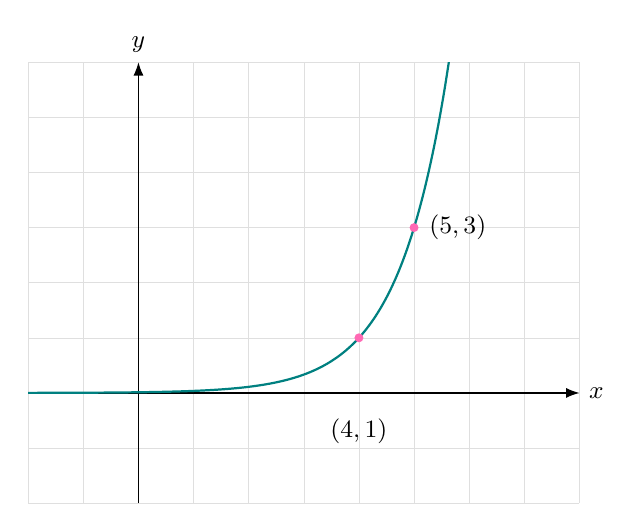
\begin{tikzpicture}[scale=0.7]
\draw[step=1, gray!25, very thin] (-2,-2) grid (8,6);
\draw[-{Latex}] (-2,0) -- (8,0) node[right] {\small $x$};
\draw[-{Latex}] (0,-2) -- (0,6) node[above] {\small $y$};
\begin{scope}
\clip (-2,-2) rectangle (8,6);
\draw[teal, thick, domain=-2:5.65, samples=80, smooth] plot (\x, {(1/81)*3^\x});
\end{scope}
\filldraw[pinkanno] (4,1) circle (2pt);
\filldraw[pinkanno] (5,3) circle (2pt);
\node[below] at (4,-0.3) {\small $(4,1)$};
\node[right] at (5.1,3) {\small $(5,3)$};
\end{tikzpicture}
\end{center}
\end{friendlyex}

\begin{solutionbox}
This is similar to the last problem. Start with $f(x)=ab^x$. Reading two points off the graph: when $x=4,\ y=1$, and when $x=5,\ y=3$:
\[
1=ab^4 \qquad \text{(Equation 1)}
\]
\[
3=ab^5 \qquad \text{(Equation 2)}
\]

Divide Equation 2 by Equation 1:
\[
\frac31=\frac{ab^5}{ab^4} \implies b=3.
\]

Substitute $b=3$ into Equation 1:
\[
1=a(3)^4 \implies 1=81a \implies a=\frac{1}{81}.
\]

\[
\boxed{f(x)=\frac{1}{81}(3)^x}
\]
\end{solutionbox}

\section*{Summary}

\begin{friendlyrule}{Key Ideas}
\begin{itemize}
    \item An exponential function has the form $f(x)=ab^x$ with $b>0,\ b\neq 1$; $a=f(0)$ is the initial value, and $b$ is the growth ($b>1$) or decay ($0<b<1$) factor.
    \item Writing $f(x)=ab^{x-h}+k$ shifts the graph of $y=ab^x$: $h$ units horizontally, $k$ units vertically, and the horizontal asymptote becomes $y=k$.
    \item Applications: compound interest $A=P(1+r/n)^{nt}$ (or $A=Pe^{rt}$ continuously), population growth $P(t)=P_0e^{rt}$, depreciation $V=V_0(1-r)^t$, and logistic growth $N=\dfrac{L}{1+ce^{-kt}}$.
    \item To determine $f(x)=ab^x$ from two data points, divide the equations to eliminate $a$ and solve for $b$, then substitute back to find $a$.
\end{itemize}
\end{friendlyrule}

\end{document}
